\documentclass[a4paper, 10pt]{article}
\usepackage[left=3.17cm, right=3.17cm, top=2.54cm, bottom=2.54cm]{geometry}
\usepackage[UTF8]{ctex}

\usepackage{amsmath}
\usepackage{amssymb}

\usepackage{graphicx, subfigure}
\usepackage{minted}
\setmonofont[]{Fira Code}

\usepackage{booktabs}

\title{DSP 大作业报告\\——北斗扩频信号捕获}
\author{暮月}

\begin{document}
\maketitle

\section{信号捕获原理}

简化后的扩频信号为:

\begin{align}
    s_i(t) & = \sum_{n=0}^{\infty} c_i(t - n\cdot NT_c) \\
    c_i(t) & = \sum_{n=0}^{N-1} b_i[n]p(t-nT_c)
\end{align}

即不断循环发送伪随机序列$c_i$,长度10230。由于码速率10.23Mcps,即每1ms发送一遍序列。

经信道传输后的基带信号为:

\begin{align}
    S(t) = \sum_{i\in V} A_i s_i(t - \tau_i) + w(t)
\end{align}

出于简便处理,将$w(t)$视为零均值高斯白噪声,并考虑基带信号以$NT_C$为周期循环叠加,即:

\begin{align}
    \begin{split}
        S((t))_{NT_c} & = K \sum_{i\in V} A_i s_i((t - \tau_i))_{NT_c} + \sum_{j=0}^{K-1}w_j((t))_{NT_c}\\
        & \approx K \sum_{i\in V} A_i c_i((t - \tau_i))_{NT_c}
    \end{split}
\end{align}

由于零均值高斯白噪声互相独立,故经$K$次叠加后噪声的功率放大$K$倍,而码的功率放大为$K^2$倍,或者从时域考虑叠加多次后趋于均值0。故可以使用这种方法进行去噪。

注意到叠加后的信号基本只由互相基本正交的伪随机序列码组成,故只需要对信号和63个码做时域相关,即可得到是否存在该序列和时延。但由于信号使用51.15MHz进行采样,故需要先对伪随机序列进行升采样,再进行相关运算。

\section{设计思路}

根据上一节所描述的信号捕获原理,可以得到如图\ref{fig:system}所示的信号捕获流程。

\begin{figure}[ht]
    \centering
    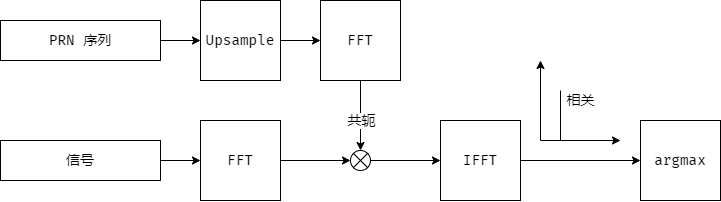
\includegraphics[width=.8\textwidth]{../assets/system.png}
    \caption{信号捕获流程}
    \label{fig:system}
\end{figure}

由于实验的信号采样率51.15MHz,码速率10.23Mcps,恰好为5倍的关系,故可以凭借先验信息对码序列进行5倍的理想升采样。即对$[1, -1]$可以升采样为$[1,1,1,1,1,-1,-1,-1,-1,-1]$。流程中还使用FFT对信号进行处理,在频域进行相乘的操作来代替时域的相关,以减小计算复杂度。需指出的是,图\ref{fig:system}中的“信号”是截取的信号片段经过周期叠加后的序列,具体截取长度根据需要可以进行调整。由上节的分析,欲得到信噪比更大的结果需要截取更长的片段进行周期叠加,但这种方法会增大系统的时延。在下节中将看到,对于本实验截取10个周期便可以得到足够好的结果,即系统除了计算的时延外仅需延时10ms以采样得到足够的数据进行处理。

对于图\ref{fig:system}所描述的捕获流程,记n种PRN序列长度N,信号长度5kN,只需5nN + 5N个复数的存储空间即可(可以直接使用计算结果覆盖信号存储的空间)。而完全在时域计算相关需5nN + 5N + 10N(使用10N个复数的空间存储时域相关结果)。同时FFT可以极大地减小计算的时间复杂度,时域计算5N点两序列相关的复数乘法复杂度$O(N^2)$,而经过FFT后计算的复杂度为$O(N\log N)$(频域乘法为$O(N)$)。故这种方法的时间复杂度和空间复杂度都优于时域直接计算相关。

\section{结果分析}

使用10ms的Task2数据,将数据周期叠加后除以10进行功率的归一,经过上节所述捕获流程得到63个相关波形于图\ref{fig:corr},可以看到有四个非常明显的相关峰。

\begin{figure}[htb]
    \centering
    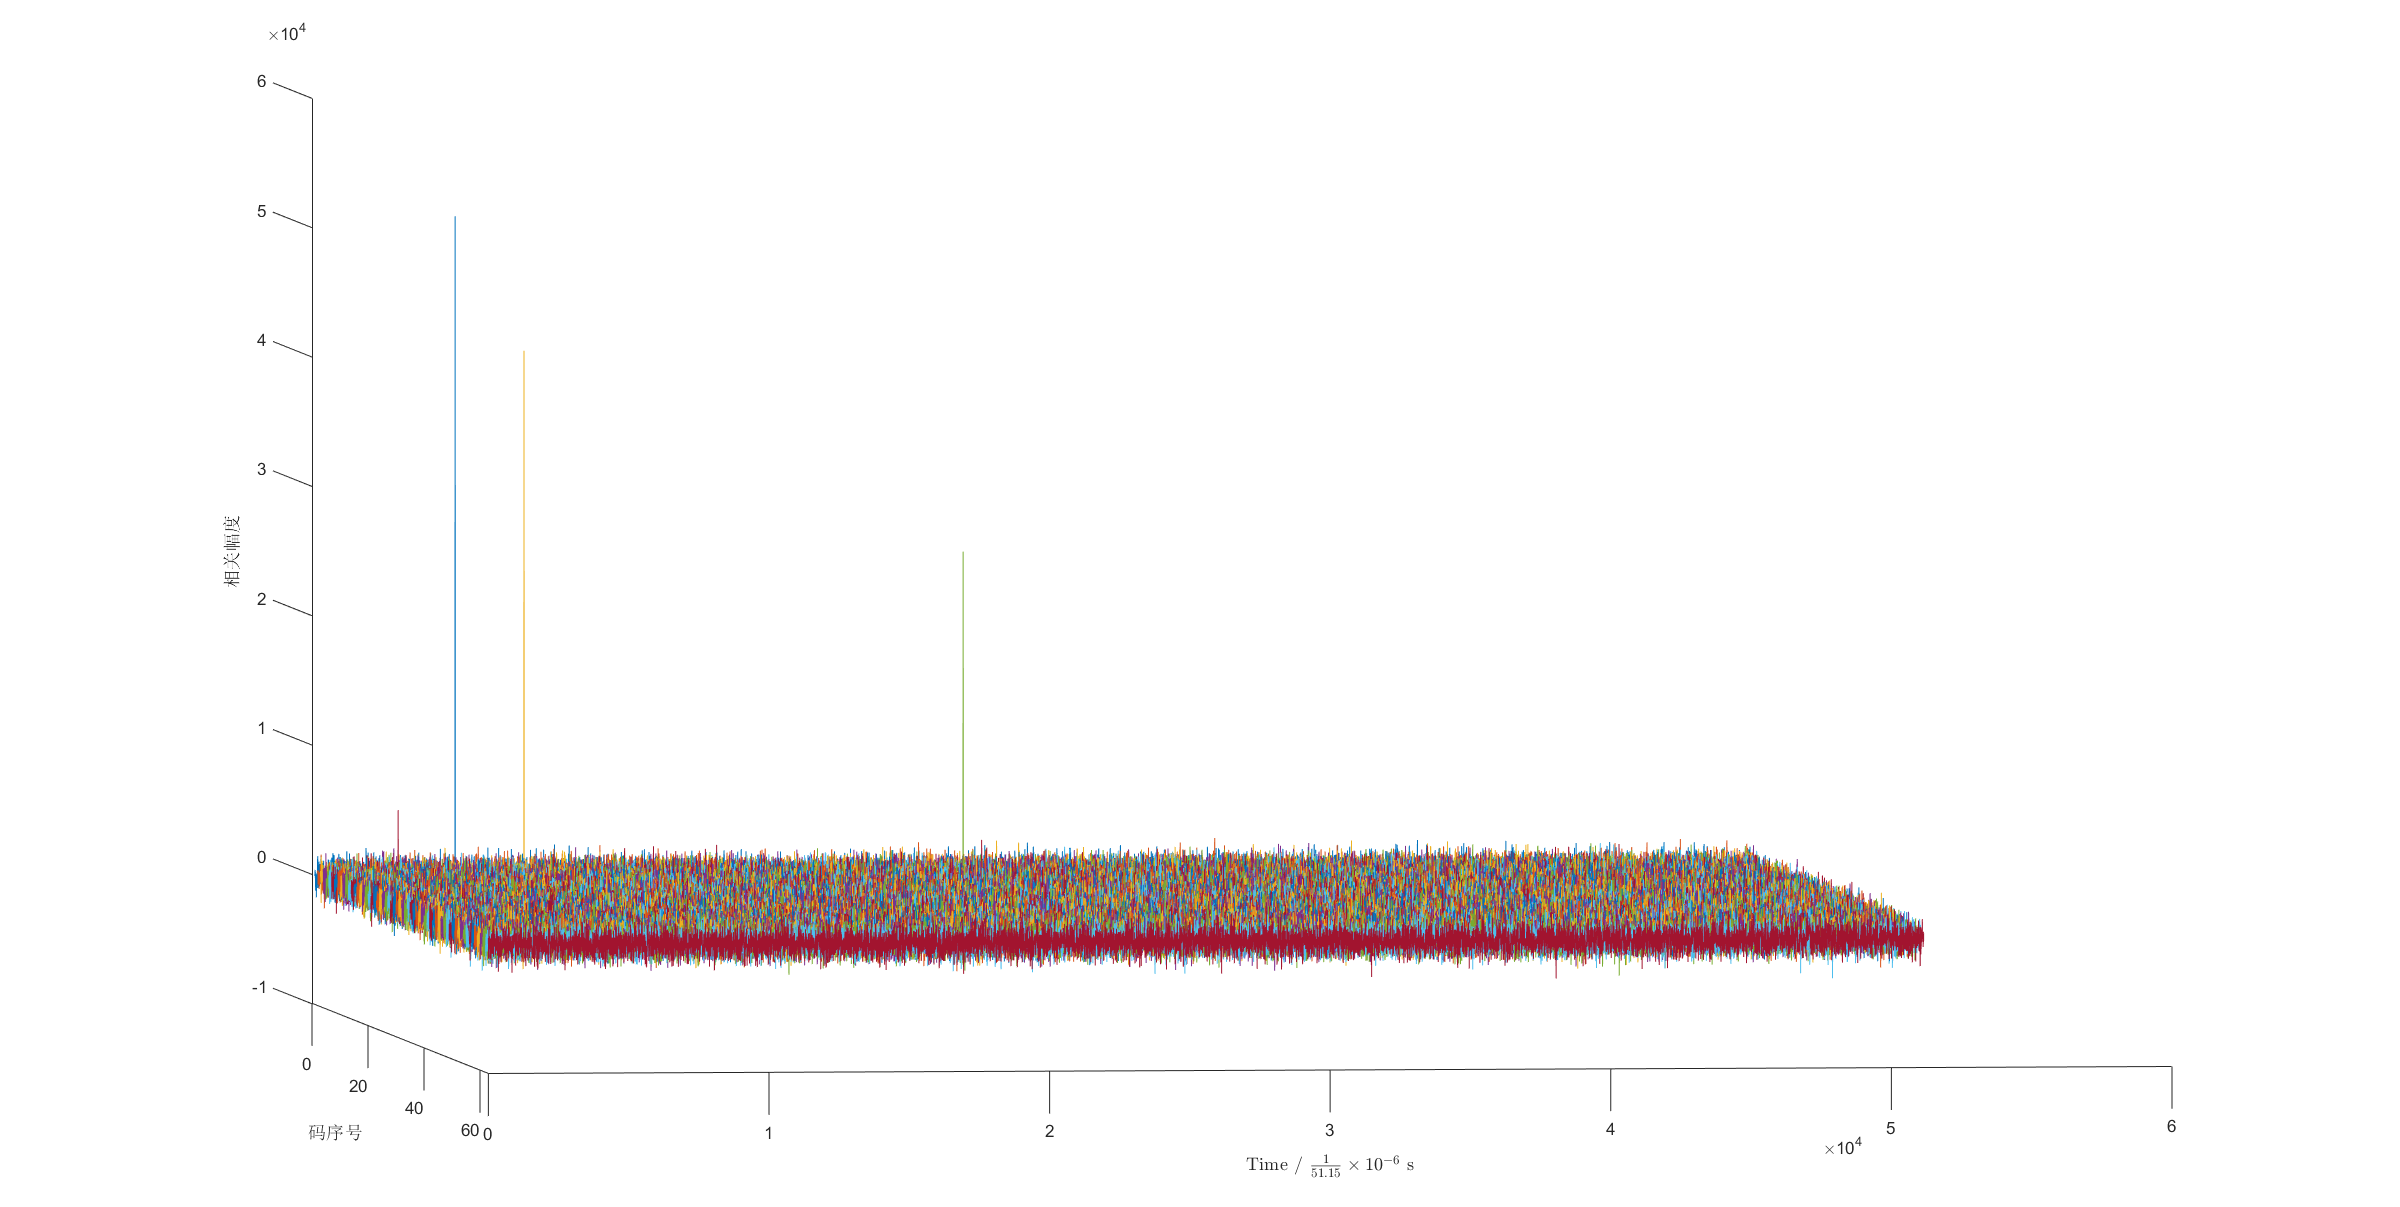
\includegraphics[width=.9\textwidth]{../assets/corr.png}
    \caption{Task2.dat与PRN码的相关波形}
    \label{fig:corr}
\end{figure}

经过对数据的观察后,使用5000作为阈值对信号进行初筛,再使用\mintinline{matlab}{max}函数找出最大值、所在码序号、所在序列位置,并将序列位置转为以10230为单位,得到表\ref{tab:delay1}。这便是图\ref{fig:corr}中四条相关峰所在的码序列和它们的位置。

\begin{table}[ht]
    \centering
    \caption{捕获强信号时延}
    \label{tab:delay1}
    \begin{tabular}{cc}
        \toprule
        码序号 & 时延(码片) \\
        \midrule
        1      & 1000         \\
        3      & 1451         \\
        5      & 4541         \\
        7      & 474          \\
        \bottomrule
    \end{tabular}
\end{table}

下面研究强度较弱的信号的捕获,图\ref{fig:corr_15}中展示了不同长度信号和15号码的相关波形,可以看到图\ref{fig:corr_15_1}的噪声较大,而使用较长的信号可以将噪声抑制在2000及以下。

\begin{figure}[ht]
    \centering
    \subfigure[1ms信号\label{fig:corr_15_1}]{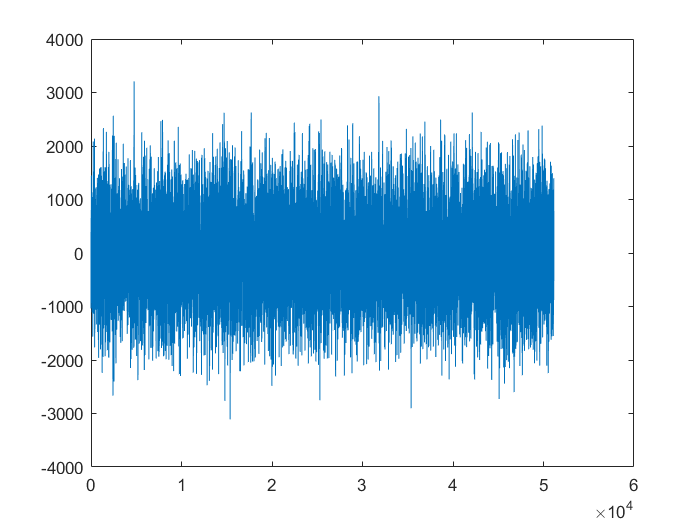
\includegraphics[width=.3\textwidth]{../assets/corr15_1}}
    \subfigure[10ms信号\label{fig:corr_15_10}]{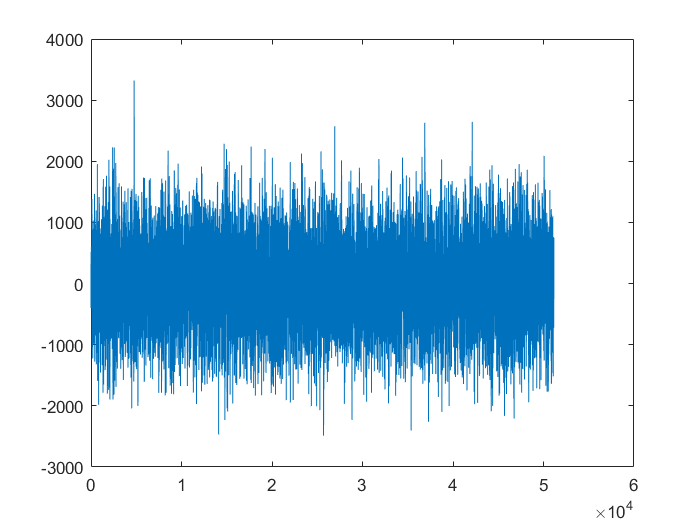
\includegraphics[width=.3\textwidth]{../assets/corr15_10}}
    \subfigure[1s信号\label{fig:corr_15_1000}]{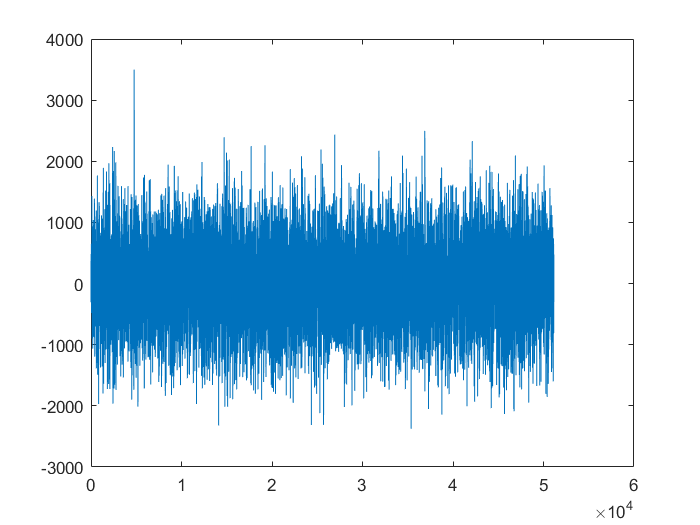
\includegraphics[width=.3\textwidth]{../assets/corr15_1000}}
    \caption{不同长度信号与15号码的相关波形}
    \label{fig:corr_15}
\end{figure}

故可以降低阈值到3000以捕获较弱的卫星信号,同时适当增加时长到100ms以提升捕获的精确度。如果信号长度较短,比如10ms甚至1ms,则会多捕获一些信号,但经一一查看认为更有可能是噪声而非信号。而1000ms则过长,且并未比100ms有明显的提升。故最终认为100ms比较合适,捕获到的信号及时延列于表\ref{tab:delay2}。

\begin{table}[ht]
    \centering
    \caption{捕获弱信号时延}
    \label{tab:delay2}
    \begin{tabular}{cc}
        \toprule
        码序号 & 时延(码片) \\
        \midrule
        1      & 1000         \\
        3      & 1451         \\
        5      & 4541         \\
        7      & 474          \\
        15     & 954          \\
        19     & 6448         \\
        27     & 5509         \\
        32     & 6988         \\
        51     & 9656         \\
        \bottomrule
    \end{tabular}
\end{table}

在上面的尝试中,仅通过调整信号筛查的阈值和采用的信号长度来捕获弱信号,可能会多捕获一些噪声,可能需尝试对噪声进一步滤除以得到更准确的结果。此外,尝试使用窗函数后发现效果不如当前的直接截断(等效矩形窗)。

\end{document}